% !TEX TS-program = xelatex
% !TEX encoding = UTF-8 Unicode
% !Mode:: "TeX:UTF-8"
\documentclass[bachelor,nocolorlinks, printoneside]{seuthesis} % 本科
% \documentclass[master]{seuthesis} % 硕士
% \documentclass[doctor]{seuthesis} % 博士
% \documentclass[engineering]{seuthesis} % 工程硕士
\usepackage{CJK,CJKnumb}
\usepackage{amsmath}
\usepackage{amsfonts}
\usepackage{bm}
\usepackage{algorithm}
\usepackage{algorithmicx}
\usepackage{algpseudocode}
\usepackage{subfigure}
\usepackage{booktabs} % 表格横线

\floatname{algorithm}{算法}
\renewcommand{\algorithmicrequire}{\textbf{输入:}}
\renewcommand{\algorithmicensure}{\textbf{输出:}}

\begin{document}

\pagestyle{seuabstractstyle}
\begin{abstract}{关键词1,关键词2,关键词3,关键词4}

摘要内容独立于正文而存在,是论文内容高度概括的简要陈述,应准确、具体、完整地概括论文的主要信息,内容包括研究目的、方法、过程、成果、结论及主要创新之处等,不含图表,不加注释,具有独立性和完整性,一般为400字左右。

“摘要”用三号黑体加粗居中,“摘”与“要”之间空4个半角空格。摘要正文内容用小四号宋体,固定1.5倍行距。

论文的关键词是反映毕业设计(论文)主题内容的名词,一般为3-5个,排在摘要正文部分下方。关键词与摘要之间空一行。关键词之间用逗号分开,最后一个关键词后不加标点符号。
\end{abstract}

\begin{englishabstract}{ Keywords1, Keywords2, Keywords3, Keywords4}

英文摘要应与中文摘相对应,250个实词左右。采用第三人称介绍该学位论文内容,叙述的基本时态为一般现在时,确实需要强调过去的事情或者已经完成的行为才使用过去时、完成时等其他时态。

ABSTRACT为三号Times New Roman加粗居中。

英文摘要正文为小四号Times New Roman,固定1.5倍行距。英文关键词“KEY WORDS”大写,其后的关键词第一个字母大写,关键词之间用半角逗号隔开。

Your abstract Your abstract Your abstract Your abstract Your abstract Your abstract Your abstract Your abstract Your abstract Your abstract Your abstract Your abstract Your abstract Your abstract Your abstract Your abstract Your abstract Your abstract Your abstract Your abstract Your abstract Your abstract Your abstract Your abstract. Your abstract Your abstract Your abstract Your abstract Your abstract Your abstract Your abstract Your abstract Your abstract Your abstract Your abstract Your abstract Your abstract Your abstract Your abstract Your abstract Your abstract Your abstract Your abstract Your abstract Your abstract Your abstract Your abstract.
\end{englishabstract}

\tableofcontents

\begin{Main} % 开始正文

\chapter{绪论}

\section{课题背景和意义}

绪论部分主要论述选题的意义、国内外研究现状以及本文主要研究的内容、研究思路以及内容安排等。

章标题为三号黑体加粗居中;一级节标题(如,2.1 本文研究内容):四号黑体居左;二级节标题(如,2.1.1 实验方法):小四号宋体居左。

正文部分为小四号宋体,行间距1.5倍行距,首行缩进2个字符。

\subsection{subsection}
。。。。。

\section{研究现状}
……

\section{本文研究内容}
……

\chapter{正文}

正文部分每一章应另起页书写书写,层次要清楚,内容要有逻辑性,正文一般不少于15000字。正文部分因学科、选题特点可有差异,但必须言之成理,论据可靠,严格遵循本学科国际通行的学术规范。

中文为小四号宋体,英文及数字为小四号Times New Roman,首行缩进2个字符,行间距为1.5倍。

\section{插图格式要求}

插图力求精炼,且每个插图均应有图序和图名。图序与图名位于插图下方,图序一般按章节编排,如图1-1(第一章第1个图),在插图较少时可以全文连续编序,如图10。

如一个插图由两个及以上的分图组成,分图用(a)、(b)、(c)等标出,并标出分图名。

简单文字图可用WORD直接绘制,复杂的图考虑使用相应的图形绘制软件完成,以提高图形表达质量。

插图居中排列,与上文文本之间空一行。图序图名设置为五号宋体居中,图序与图名之间空一格。

\begin{figure}[!htbp]
\centering
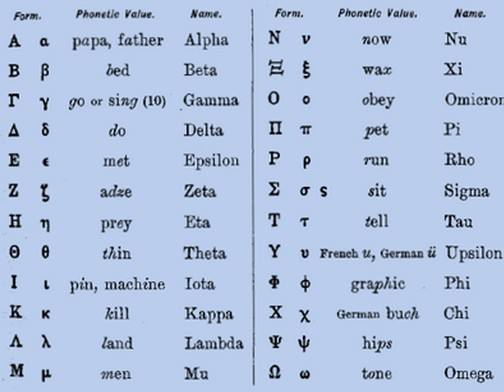
\includegraphics[width=0.5\textwidth]{img/test.jpg} \caption{图片的一个简单应用场景}
\end{figure}

\begin{figure}[!htbp]
\centering
\subfigure[the first subfigure]{
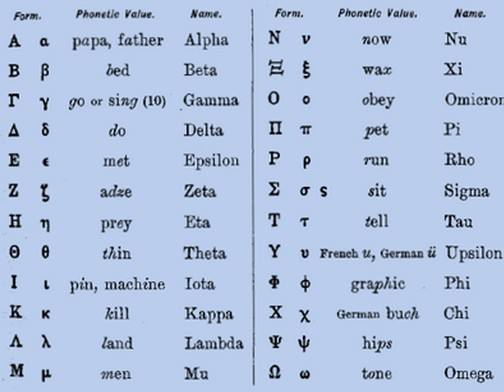
\includegraphics[width=0.3\textwidth]{img/test.jpg} 
}
\subfigure[the second subfigure]{
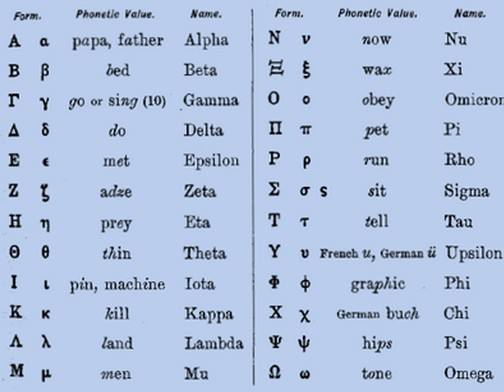
\includegraphics[width=0.3\textwidth]{img/test.jpg} 
}
\caption{子图应用场景}
\end{figure}

\section{表格格式要求}

表格的结构应简洁,一律采用三线表,应有表序和表名,且表序和表名位于表格上方。表格可以逐章单独编序(如:表2.1),也可以统一编序(如:表10),采用哪种方式应和插图及公式的编序方式统一。表序必须连续,不得重复或跳跃。

表格无法在同一页排版时,可以用续表的形式另页书写,续表需在表格右上角表序前加“续”字,如“续表2.1”,并重复表头。

表格居中,边框为黑色直线1磅,中文为五号宋体,英文及数字为五号Times New Roman字体,表序与表名之间空一格,表格与下文之间空一行。

\begin{table}[htbp]
    \caption{降水率分级统计} 
    \centering
	\wuhao
    \begin{tabular}{ccc} 
%        \toprule[1pt]
		\hline
        降水率(mm/h)分级 & 该等级所占比例(\%) & 降水等级描述  \\
%        \midrule[1pt]
		\hline
        $0\le x\le 0.5$& 90.36 & 没有雨或雨很小 \\
        ... & ...&....  \\
%        \bottomrule[1pt]
		\hline
\end{tabular}\end{table}

\section{表达式}
\begin{equation}
a^2+b^2=c^2\label{勾股定理}
\end{equation}

勾股定理(\ref{勾股定理})。

\section{注释}

注释\footnote{脚注内容}

\section{引用论文}
使得论文符合要求\cite{Yao:2015ix}\cite{seucover}\cite{test1}\cite{test}\cite{R1}。

% 参考文献
\bibliography{seuthesis}

% 附录
\begin{Appendix}
\chapter{附录标题}
附录正文
\end{Appendix}

\begin{Acknowledgement}{}
这次的毕业论文设计总结是在我的指导老师xxx老师亲切关怀和悉心指导下完成的。从毕业设计选题到设计完成,x老师给予了我耐心指导与细心关怀,有了莫老师耐心指导与细心关怀我才不会在设计的过程中迷失方向,失去前进动力。x老师有严肃的科学态度,严谨的治学精神和精益求精的工作作风,这些都是我所需要学习的,感谢x老师给予了我这样一个学习机会,谢谢!

感谢与我并肩作战的舍友与同学们,感谢关心我支持我的朋友们,感谢学校领导、老师们,感谢你们给予我的帮助与关怀;感谢肇庆学院,特别感谢计算机科学与软件学院四年来为我提供的良好学习环境,谢谢!
\end{Acknowledgement}

\newpage
\printindex % 索引

\end{Main} % 结束正文

%\begin{thebibliography}{99}


%\bibliographystyle{ieee}
%\bibliography{seuthesis}


\end{document}
